\documentclass[output=paper,colorlinks,citecolor=brown]{langscibook} 

\newcommand*{\fullref}[1]{\hyperref[{#1}]{\autoref*{#1}: \nameref*{#1}}} % One single link

%dependencias para desenhar árvores sintáticas
\usepackage{tikz}
\usepackage{tikz-dependency}
%\usepackage{python}
%\usepackage{minted} %\begin{minted}{python}
\usepackage{longtable}

%nome da section no header de cada página
%\usepackage{fancyhdr}
%\pagestyle{fancy}
%\fancyhf{}
%\fancyhead[L]{\rightmark}
%\fancyhead[R]{\thepage}
%\renewcommand{\headrulewidth}{0pt}
\usepackage{dirtytalk}

\bibliography{localbibliography.bib}

\author{Elvis de Souza\affiliation{PUC-Rio, Brasil}\and Tatiana Cavalcanti\and Aline Silveira\and Wograine Evelyn\and Cláudia Freitas}
\title{Documentação UD em português\\
(e para língua portuguesa)}
\abstract{O projeto Universal Dependencies \citep{mcdonald2013universal} apresenta um tagset e uma gramática. Isso significa dizer que, para além de um conjunto de etiquetas que correspondem às classes da Gramática Tradicional (objeto, sujeito etc.), o UD também faz diversas escolhas que diferem da GT. Nesse documento, apresentamos a documentação detalhadas e as escolhas linguísticas relativas ao processo de revisão do material UD em Português. Considerando que UD funciona como uma espécie de segunda língua gramatical, partimos, sempre que possível, das categorias e análises de GT, e não de UD. Os exemplos de frases e as listas foram retirados do corpus \href{https://github.com/UniversalDependencies/UD\_Portuguese-Bosque}{Bosque-UD} (\citet{rademaker2017universal}) versão 2.5.}

% add all extra packages you need to load to this file  
\usepackage{tabularx} 

%%%%%%%%%%%%%%%%%%%%%%%%%%%%%%%%%%%%%%%%%%%%%%%%%%%%
%%%                                              %%%
%%%           Examples                           %%%
%%%                                              %%%
%%%%%%%%%%%%%%%%%%%%%%%%%%%%%%%%%%%%%%%%%%%%%%%%%%%% 
%% to add additional information to the right of examples, uncomment the following line
% \usepackage{jambox}
%% if you want the source line of examples to be in italics, uncomment the following line
% \renewcommand{\exfont}{\itshape}
\usepackage{langsci-optional}
\usepackage{langsci-gb4e}  
\makeatletter
\let\thetitle\@title
\let\theauthor\@author 
\makeatother

\newcommand{\togglepaper}[1][0]{ 
%   \bibliography{../localbibliography}
  \papernote{\scriptsize\normalfont
    \theauthor.
    \thetitle. 
    To appear in: 
    Change Volume Editor \& in localcommands.tex 
    Change volume title in localcommands.tex
    Berlin: Language Science Press. [preliminary page numbering]
  }
  \pagenumbering{roman}
  \setcounter{chapter}{#1}
  \addtocounter{chapter}{-1}
}

\begin{document}

\maketitle

\addtocontents{toc}{\protect\hypertarget{toc}{}}

\tableofcontents

\chapter{Formato UD}\label{sec:formatoud}

\hyperlink{toc}{Ir para tabela de conteúdos\\}

Os treebanks adaptados para a gramática UD são disponibilizados no formato CoNLL, em que há um token por linha. Cada anotação de cada token, por sua vez, é disposta em uma coluna, sendo 10 colunas ao todo. Cada token tem a configuração conforme a \fullref{tab:colunasUD}, com uma tabulação (\textit{Tab}) separando as colunas. Colunas sem nenhum valor devem, necessariamente, ser preenchidas com \textit{underline}.

\begin{table}
    \centering
    \begin{tabular}{c c c c c c c c c c}
        id & word & lemma & upos & xpos & feats & dephead & deprel & deps & misc\\
    \end{tabular}
    \caption{Colunas do formato UD 2.0}
    \label{tab:colunasUD}
\end{table}

\section{Colunas/anotações}\label{sec:colunas}



\begin{enumerate}
    \item “id” corresponde ao número do token, em ordem crescente;
    \item “word”, à palavra tal como aparece na frase (exceto no caso de contração, como “da”, em que a palavra será desmembrada nos tokens “de” e “a”);
    \item “lemma” se refere à palavra tal como aparece no dicionário: em no singular e em masculino ou infinitivo;
    \item “upos” (classe gramatical \say{universal}) se refere à classe gramatical;
    \item No corpus Bosque-UD, a coluna “xpos” (classe gramatical específica) é preenchida com a saída do sistema PALAVRAS para a mesma frase;
    \item “feats” (atributos morfológicos) é preenchida com as características morfológicas do token;
    \item “dephead” (dependência sintática), com o id do token de quem é filho;
    \item “deprel” (relação de dependência), com a relação sintática que o conecta ao seu pai;
    \item “deps” (dependência específica) não é utilizado no Bosque-UD;
    \item “misc” (miscelânea) se refere a quaisquer informações extras que desejemos adicionar ao token.
\end{enumerate}{}

\section{Manipulação em Python}\label{sec:python}



Para manipular arquivos no formato UD em Python, com as classes Corpus, Sentence e Token (e suas respectivas anotações), desenvolvemos e utilizamos o \href{https://github.com/alvelvis/ACDC-UD/blob/master/estrutura_ud.py}{estrutura\_ud.py}.

\chapter{Classes gramaticais (upos)}\label{sec:upos}

\hyperlink{toc}{Ir para tabela de conteúdos\\}



As classes gramaticais em UD podem ser consultadas na \fullref{tab:upos}.

\begin{table}[]
    \centering
    \begin{tabular}{| c | c |}
    \hline
    \textbf{upos} & \textbf{Observações} \\
    \hline
    ADJ & adjetivos e numerais ordinais \\
    \hline
    ADP & preposições \\
    \hline
    PUNCT & pontuação \\
    \hline
    ADV & advérbio \\
    \hline
    AUX & \fullref{sec:verbosauxiliares} \\
    \hline
    SYM & símbolos \\
    \hline
    INTJ & interjeição \\
    \hline
    CCONJ & conjunção coordenativa \\
    \hline
    NOUN & substantivo \\
    \hline
    DET & determinante - artigos e pronomes adjetivos \\
    \hline
    PROPN & nomes próprios, apenas se com inicial maiúscula \\
    \hline
    NUM & numeral - exceto os ordinais, que são adjetivos \\
    \hline
    PART & partícula \\
    \hline
    VERB & verbo \\
    \hline
    PRON & apenas pronomes substantivos \\
    \hline
    SCONJ & conjunções subordinativas \\
    \hline
    X & no Bosque-UD, palavras estrangeiras \\
    \hline
    \end{tabular}
    \caption{As classes gramaticais do UD em português}
    \label{tab:upos}
\end{table}{}



\section{Verbos auxiliares}\label{sec:verbosauxiliares}

	Verbos auxiliares são classificados como \emph{AUX}. O que conta como um verbo auxiliar é alvo de discussão nas gramáticas do português (\citet{elvis2019locverbal}). De modo geral, classificamos como verbos auxiliares os verbos de ligação (\fullref{sec:verbosdeligação}), o verbo auxiliar na voz passiva (\fullref{sec:servozpassiva}), as locuções de tempo composto (\fullref{sec:auxtempocomposto}), e as locuções verbais aspectuais e modais (\fullref{sec:auxaspecto}).
	
	Via de regra, verbos auxiliares (\emph{AUX}) não podem ter dependentes, e dependem de um verbo principal (\emph{VERB}). O deprel pode ser \emph{cop}, \emph{aux} ou \emph{aux:pass}, de acordo com a função sintática.

	A \fullref{tab:aux} mostra a lista com todos os verbos auxiliares, sejam eles verbos de ligação, voz passiva ou locuções verbais de tempo composto/aspectuais/modais.

	A \fullref{tab:verbosdeligação} mostra a lista apenas com os verbos de ligação.

	A \fullref{tab:vozpassiva} mostra a lista de todos os verbos que ocupam a posição de voz passiva.

	A \fullref{tab:locuçõesverbais} mostra a lista de todos os verbos que são auxiliares em uma locução verbal.

	\begin{table}[]
		\parbox{.45\linewidth}{
			\centering
			\begin{tabular}{|c|c|}
				\hline
				\textbf{Verbo auxiliar} & \textbf{Frequência} \\\hline
					acabar & 56\\\hline
					andar & 4\\\hline
					chegar & 19\\\hline
					começar & 62\\\hline
					continuar & 57\\\hline
					costumar & 10\\\hline
					deixar & 24\\\hline
					dever & 217\\\hline
					estar & 282\\\hline
					faltar & 1\\\hline
					ficar & 11\\\hline
					haver & 37\\\hline
					ir & 358\\\hline
					parar & 3\\\hline
					parecer & 17\\\hline
					passar & 39\\\hline
					poder & 394\\\hline
					procurar & 1\\\hline
					quer & 1\\\hline
					ser & 1304\\\hline
					ter & 536\\\hline
					vir & 68\\\hline
					voltar & 40\\\hline
			\end{tabular}
		}
		\hfill
		\parbox{.45\linewidth}{
			\centering
			\begin{tabular}{|c|c|}
				\hline
				\textbf{Verbo auxiliar} & \textbf{Frequência} \\\hline
					ser & 1304\\\hline
					ter & 536\\\hline
					poder & 394\\\hline
					ir & 358\\\hline
					estar & 282\\\hline
					dever & 217\\\hline
					vir & 68\\\hline
					começar & 62\\\hline
					continuar & 57\\\hline
					acabar & 56\\\hline
					voltar & 40\\\hline
					passar & 39\\\hline
					haver & 37\\\hline
					deixar & 24\\\hline
					chegar & 19\\\hline
					parecer & 17\\\hline
					ficar & 11\\\hline
					costumar & 10\\\hline
					andar & 4\\\hline
					parar & 3\\\hline
					faltar & 1\\\hline
					procurar & 1\\\hline
					quer & 1\\\hline
			\end{tabular}
		}
		\caption{Lista das 23 palavras que ocorrem 3541 vezes como verbo auxiliar no Bosque-UD}
		\label{tab:aux}
	\end{table}

	\begin{table}[]
		\centering
		\begin{tabular}{|c|c|}
			\hline
			\textbf{Verbo de ligação} & \textbf{Frequência} \\\hline
			estar & 33\\\hline
			ser & 105\\\hline
		\end{tabular}
		\caption{Lista das 2 palavras que ocorrem 138 vezes como verbo de ligação no Bosque-UD}
		\label{tab:verbosdeligação}
	\end{table}

	\begin{table}[]
		\centering
		\begin{tabular}{|c|c|}
			\hline
			\textbf{Voz passiva} & \textbf{Frequência} \\\hline
			ficar & 1\\\hline
			ser & 1114\\\hline
		\end{tabular}
		\caption{Lista das 2 palavras que ocorrem 1115 vezes como voz passiva no Bosque-UD}
		\label{tab:vozpassiva}
	\end{table}

	\begin{table}[]
		\parbox{.45\linewidth}{
			\centering
			\begin{tabular}{|c|c|}
				\hline
				\textbf{Locução verbal} & \textbf{Frequência} \\\hline
				acabar & 56\\\hline
				andar & 4\\\hline
				chegar & 19\\\hline
				começar & 62\\\hline
				continuar & 57\\\hline
				costumar & 10\\\hline
				deixar & 24\\\hline
				dever & 217\\\hline
				estar & 249\\\hline
				faltar & 1\\\hline
				ficar & 10\\\hline
				haver & 37\\\hline
				ir & 358\\\hline
				parar & 3\\\hline
				parecer & 17\\\hline
				passar & 39\\\hline
				poder & 394\\\hline
				procurar & 1\\\hline
				quer & 1\\\hline
				ser & 53\\\hline
				ter & 536\\\hline
				vir & 68\\\hline
				voltar & 40\\\hline
			\end{tabular}
		}
		\hfill
		\parbox{.45\linewidth}{
			\centering
			\begin{tabular}{|c|c|}
				\hline
				\textbf{Locução verbal} & \textbf{Frequência} \\\hline
				ter & 536\\\hline
				poder & 394\\\hline
				ir & 358\\\hline
				estar & 249\\\hline
				dever & 217\\\hline
				vir & 68\\\hline
				começar & 62\\\hline
				continuar & 57\\\hline
				acabar & 56\\\hline
				ser & 53\\\hline
				voltar & 40\\\hline
				passar & 39\\\hline
				haver & 37\\\hline
				deixar & 24\\\hline
				chegar & 19\\\hline
				parecer & 17\\\hline
				costumar & 10\\\hline
				ficar & 10\\\hline
				andar & 4\\\hline
				parar & 3\\\hline
				faltar & 1\\\hline
				procurar & 1\\\hline
				quer & 1\\\hline
			\end{tabular}
		}
		\caption{Lista das 23 palavras que ocorrem 2256 vezes como locução verbal no Bosque-UD}
		\label{tab:locuçõesverbais}
	\end{table}

	\subsection{Verbos de ligação}\label{sec:verbosdeligação}
	
		Apenas os verbos \say{ser} e \say{estar} são considerados verbos de ligação, e portanto serão sempre anotados como \textit{AUX}. Os demais verbos que a GT costuma elencar como verbo de ligação (parecer, permanecer, etc.) são anotados como \textit{VERB}. Os verbos de ligação \textit{AUX} terão relação sintática \emph{cop}, e nunca poderão ser núcleo de uma oração (Xx) nem conter dependentes. \fullref{dep:serAUX}.

		A frequência dos verbos de ligação pode ser consultada em \fullref{tab:verbosdeligação}.
		
		\begin{figure*}[htbp]
		    \centering
		    \vspace{.8cm}
		    \begin{dependency}
		    \begin{deptext}
		    DET \& NOUN \& AUX \& ADP \& SYM \& NUM \\
		    O \& preço \& é \& de \& US\$ \& 422 \\
		    o \& preço \& ser \& de \& US\$ \& 422 \\
		    \end{deptext}
		    \depedge{2}{1}{det}
		    \deproot{5}{root}
		    \depedge{5}{2}{nsubj}
		    \depedge{5}{3}{cop}
		    \depedge{5}{4}{case}
		    \depedge{5}{6}{nummod}
		    \end{dependency}
		    \caption{O preço \emph{é} de US\$ 422}\label{dep:serAUX}
		\end{figure*}


	\subsection{Verbo \textit{ser} como voz passiva}\label{sec:servozpassiva}
	
		A anotação de \say{ser} como voz passiva, além do upos \emph{AUX}, deve receber deprel \emph{aux:pass}, como na \fullref{dep:serPASS}.

		A frequência da voz passiva pode ser consultada em \fullref{tab:vozpassiva}.
		
		\begin{figure*}[htbp]
		    \centering
		    \vspace{.8cm}
		    \begin{dependency}
		    \begin{deptext}
		    DET \& NOUN \& AUX \& VERB \& ADP \& DET \& NOUN \\
		    A \& fotografia \& foi \& publicada \& em \& a \& imprensa \\
		    o \& fotografia \& ser \& publicar \& em \& a \& imprensa \\
		    \& \& \& VerbForm=Part \& \& \& \\
		    \end{deptext}
		    \depedge{2}{1}{det}
		    \depedge{4}{3}{aux:pass}
		    \deproot{4}{root}
			\depedge{4}{7}{obl}
		    \depedge{4}{2}{nsubj}
		    \depedge{7}{6}{det}
		    \depedge{7}{5}{case}
		    \end{dependency}
		    \caption{A fotografia \emph{foi} publicada na imprensa}\label{dep:serPASS}
		\end{figure*}
	

	\subsection{Locuções verbais de tempo composto}\label{sec:auxtempocomposto}

		Segundo as gramáticas, são locuções verbais de tempo composto aquelas que têm como verbo auxiliar \say{ter}, \say{haver} e, para nós, também \say{ir}. Confira um exemplo de locução verbal de tempo composto na \fullref{dep:auxtempocomposto}. 

		A \fullref{tab:locuçõesverbais} mostra a lista de locuções verbais, entre elas, as de tempo composto.

		\begin{figure*}[htbp]
			\centering
			\vspace{.8cm}
			\begin{dependency}
				\begin{deptext}
					DET \& PROPN \& ADV \& AUX \& VERB \& DET \& NOUN \& PUNCT \\
					A \& Prefeitura \& não \& havia \& retirado \& o \& golfinho \& . \\
					o \& Prefeitura \& não \& haver \& retirar \& o \& golfinho \& . \\
					\& \& Polarity=Neg \& \& \& \& \& \\
				\end{deptext}
				\depedge{2}{1}{det}
				\depedge{5}{3}{advmod}
				\deproot{5}{root}
				\depedge{5}{7}{obl}
				\depedge{5}{2}{nsubj}
				\depedge{7}{6}{det}
				\depedge{5}{7}{obj}
				\depedge{5}{8}{punct}
				\depedge{5}{4}{aux}
			\end{dependency}
			\caption{A Prefeitura não \emph{havia retirado} o golfinho}
			\label{dep:auxtempocomposto}
		\end{figure*}


	\subsection{Locuções verbais aspectuais/modais}\label{sec:auxaspecto}

		Confira um exemplo de locução verbal aspectual na \fullref{dep:auxphrasalverb}, e modal na \fullref{dep:auxmodal}.

		A \fullref{tab:locuçõesverbais} mostra a lista de locuções verbais, entre elas, as locuções verbais aspectuais/modais.

		Segundo as gramáticas, o que distingue a locução verbal aspectual da modal é que, na primeira, o verbo auxiliar caracteriza a temporalidade da ação do verbo principal, e na segunda, o verbo auxiliar caracteriza um julgamento do enunciador sobre a ação do verbo principal. Alguns gramáticos divergem sobre como a classificação se dá, portanto apenas herdamos, no Bosque-UD, o que já era a anotação originária do PALAVRAS \citep{bick2000parsing}, e resolvemos não modificá-la.

		Repare que, nos casos de locução verbal aspectual, geralmente há uma partícula interveniente no meio da locução, como na \fullref{dep:auxphrasalverb}, em que há um \say{a} entre \say{começar} e \say{ouvir}. Encaramos que estamos diante de um fenômeno de \emph{phrasal verb}, uma MWE do tipo \emph{AUX}, como sugerido em \citet{elvis2019locverbal}. Na frase, \emph{vai ouvir} é uma locução verbal de tempo composto (\fullref{sec:auxtempocomposto}), e \say{começar a ouvir} é uma locução verbal aspectual, sendo \say{começar a} uma expressão multi-palavra (MWE) do tipo auxiliar.

		Listamos essas MWEs auxiliares com partículas intervenientes na \fullref{tab:auxphrasalverb}.

		\begin{figure*}[htbp]
			\centering
			\vspace{.8cm}
			\begin{dependency}
				\begin{deptext}
					DET \& NOUN \& AUX \& VERB \& ADV \& ADP \& PROPN \& PUNCT \\
					A \& seleção \& deve \& contar \& hoje \& com \& Giovane \& . \\
					o \& seleção \& dever \& contar \& hoje \& com \& Giovane \& . \\
				\end{deptext}
				\depedge{2}{1}{det}
				\depedge{4}{5}{advmod}
				\deproot{4}{root}
				\depedge{4}{7}{obl}
				\depedge{7}{6}{case}
				\depedge{4}{2}{nsubj}
				\depedge{4}{8}{punct}
				\depedge{4}{3}{aux}
			\end{dependency}
			\caption{A seleção \emph{deve contar} hoje com Giovane}
			\label{dep:auxmodal}
		\end{figure*}

		\begin{figure*}[htbp]
			\centering
			\vspace{.8cm}
			\begin{dependency}
				\begin{deptext}
					DET \& PROPN \& AUX \& AUX \& ADP \& VERB \& DET \& NOUN \& PUNCT \\
					O \& Tribunal \& vai \& começar \& a \& ouvir \& as \& testemunhas \& . \\
					o \& Tribunal \& ir \& começar \& a \& ouvir \& o \& testemunha \& . \\
					\& \& \& \& MWE=começar\_a \& \& \& \& \\
					\& \& \& \& MWEPOS=AUX \& \& \& \& \\
				\end{deptext}
				\depedge{2}{1}{det}
				\deproot{6}{root}
				\depedge{6}{8}{obj}
				\depedge{8}{7}{det}
				\depedge{6}{2}{nsubj}
				\depedge{6}{9}{punct}
				\depedge{6}{3}{aux}
				\depedge{6}{4}{aux}
				\depedge{4}{5}{compound}
			\end{dependency}
			\caption{O Tribunal vai \emph{começar a ouvir} as testemunhas}
			\label{dep:auxphrasalverb}
		\end{figure*}

		\begin{table}[]
			\parbox{.45\linewidth}{
				\centering
				\begin{tabular}{|c|c|}
					\hline
					\textbf{MWE auxiliar} & \textbf{Frequência} \\\hline
						acabar de & 11\\\hline
						acabar por & 30\\\hline
						andar a & 3\\\hline
						chegar a & 22\\\hline
						começar a & 58\\\hline
						começar por & 6\\\hline
						continuar a & 57\\\hline
						continuar por & 1\\\hline
						deixar de & 30\\\hline
						dever a & 1\\\hline
						estar a & 124\\\hline
						estar para & 1\\\hline
						estar por & 1\\\hline
						ficar a & 4\\\hline
						ficar de & 1\\\hline
						haver a & 1\\\hline
						haver de & 2\\\hline
						haver que & 1\\\hline
						ir a & 3\\\hline
						ir de & 1\\\hline
						parar de & 3\\\hline
						passar a & 43\\\hline
						poder a & 3\\\hline
						ser de & 3\\\hline
						tender a & 1\\\hline
						ter a & 9\\\hline
						ter de & 62\\\hline
						ter que & 3\\\hline
						tornar a & 1\\\hline
						vir a & 42\\\hline
						voltar a & 42\\\hline
				\end{tabular}
			}
			\hfill
			\parbox{.45\linewidth}{
				\centering
				\begin{tabular}{|c|c|}
					\hline
					\textbf{MWE auxiliar} & \textbf{Frequência} \\\hline
						estar a & 124\\\hline
						ter de & 62\\\hline
						começar a & 58\\\hline
						continuar a & 57\\\hline
						passar a & 43\\\hline
						vir a & 42\\\hline
						voltar a & 42\\\hline
						acabar por & 30\\\hline
						deixar de & 30\\\hline
						chegar a & 22\\\hline
						acabar de & 11\\\hline
						ter a & 9\\\hline
						começar por & 6\\\hline
						ficar a & 4\\\hline
						andar a & 3\\\hline
						ir a & 3\\\hline
						parar de & 3\\\hline
						poder a & 3\\\hline
						ser de & 3\\\hline
						ter que & 3\\\hline
						haver de & 2\\\hline
						continuar por & 1\\\hline
						dever a & 1\\\hline
						estar para & 1\\\hline
						estar por & 1\\\hline
						ficar de & 1\\\hline
						haver a & 1\\\hline
						haver que & 1\\\hline
						ir de & 1\\\hline
						tender a & 1\\\hline
						tornar a & 1\\\hline
				\end{tabular}
			}
			\caption{Lista das 31 MWEs que ocorrem 570 vezes como locuções auxiliares no Bosque-UD}
			\label{tab:auxphrasalverb}
		\end{table}


	\subsection{Isso \emph{foi} nos Estados Unidos: verbo \textit{ser} como verbo pleno (\emph{VERB})}\label{sec:serpleno}
	
		Atenção para 2 casos em que o \say{ser} não é verbo auxiliar e deve ser verbo pleno (upos \textit{VERB}).
		
		1) Como na \fullref{dep:serVERB}, o \say{ser} deve ser núcleo da oração caso o predicado seja uma outra oração (\textit{ccomp, xcomp}).
		
		\begin{figure*}[htbp]
		    \centering
		    \vspace{.8cm}
		    \begin{dependency}
		    \begin{deptext}
		    DET \& NOUN \& VERB \& SCONJ \& VERB \& ADP \& SYM \& NUM \& NUM \\
		    A \& expectativa \& era \& que \& chegasse \& a \& US\$ \& 7 \& milhões \\
		    o \& expectativa \& ser \& que \& chegar \& a \& US\$ \& 7 \& milhão \\
		    \& \& \& \& \& \& \& MWE=7\_milhões \& \\
		    \& \& \& \& \& \& \& MWEPOS=NUM \& \\
		    \end{deptext}
		    \depedge{2}{1}{det}
		    \depedge{3}{2}{nsubj}
		    \deproot{3}{root}
		    \depedge{3}{5}{ccomp}
		    \depedge{5}{4}{mark}
		    \depedge{7}{6}{case}
		    \depedge{8}{9}{flat}
		    \depedge{7}{8}{nummod}
		    \depedge{5}{7}{obl}
		    \end{dependency}
		    \caption{A expectativa \emph{era} que chegasse a US\$7 milhões}\label{dep:serVERB}
		\end{figure*}
		
		2) \say{ser} verbo intransitivo (verbo pleno) também deve ter a anotação \textit{VERB}, como na \fullref{dep:serVERB2}.
		
		\begin{figure*}[htbp]
		    \centering
		    \vspace{.8cm}
		    \begin{dependency}
		    \begin{deptext}
		    PRON \& VERB \& ADP \& DET \& PROPN \& PROPN \\
		    Isso \& foi \& em \& os \& Estados \& Unidos \\
		    isso \& ser \& em \& o \& Estados \& Unidos \\
		    \& \& \& \& MWE=Estados\_Unidos \& \\
		    \& \& \& \& MWEPOS=PROPN \& \\
		    \end{deptext}
		    \depedge{2}{1}{nsubj}
		    \depedge{5}{3}{case}
		    \deproot{2}{root}
		    \depedge{5}{4}{det}
		    \depedge{5}{6}{flat:name}
		    \depedge{2}{5}{obl}
		    \end{dependency}
		    \caption{Isso \emph{foi} nos Estados Unidos}\label{dep:serVERB2}
		\end{figure*}


	\subsection{Não são locuções verbais: \emph{VERB + VERB}}

		Ainda segundo as decisões do PALAVRAS \citep{bick2000parsing}, há outras tantas colocações de dois verbos que não são locuções verbais. Portanto, são todos casos de verbos plenos, de upos \emph{VERB}, em que o segundo verbo é dependente do primeiro, como oração substantiva objetiva reduzida de infinitivo (Xx). Veja a lista de verbos na \fullref{tab:nãolocverbal}.

		\begin{longtable}{ p{3cm} | p{1cm} | p{3cm} | p{1cm} }
			\hline
			\textbf{Primeiro verbo (ordem alfabética)} & \textbf{\#} & \textbf{Primeiro verbo (ordem de frequência)} & \textbf{\#} \\\hline
			abster & 2 & querer & 108\\\hline
			acabar & 3 & conseguir & 83\\\hline
			aceder & 1 & tentar & 64\\\hline
			aceitar & 6 & fazer & 45\\\hline
			achar & 5 & pretender & 39\\\hline
			aconselhar & 5 & permitir & 37\\\hline
			acreditar & 2 & decidir & 33\\\hline
			acusar & 30 & acusar & 30\\\hline
			admitir & 12 & deixar & 27\\\hline
			afirmar & 13 & procurar & 21\\\hline
			aguentar & 1 & levar & 20\\\hline
			ajudar & 9 & ver & 19\\\hline
			alegar & 3 & dar & 18\\\hline
			ambicionar & 1 & gostar & 17\\\hline
			ameaçar & 14 & obrigar & 17\\\hline
			andar & 2 & ser & 17\\\hline
			anunciar & 2 & saber & 16\\\hline
			aperceber & 1 & ameaçar & 14\\\hline
			apetecer & 1 & precisar & 14\\\hline
			aplicar & 1 & preferir & 14\\\hline
			apostar & 1 & resolver & 14\\\hline
			aprender & 5 & afirmar & 13\\\hline
			apresentar & 2 & admitir & 12\\\hline
			apressar & 1 & considerar & 12\\\hline
			aprestar & 1 & encontrar & 12\\\hline
			aproveitar & 1 & ter & 12\\\hline
			arriscar & 2 & dizer & 11\\\hline
			atender & 1 & destinar & 10\\\hline
			atrever & 1 & limitar & 10\\\hline
			autorizar & 3 & ajudar & 9\\\hline
			avisar & 1 & ficar & 9\\\hline
			bastar & 3 & preparar & 9\\\hline
			caber & 1 & esperar & 8\\\hline
			cansar & 1 & pensar & 8\\\hline
			cessar & 1 & comprometer & 7\\\hline
			chamar & 4 & consistir & 7\\\hline
			citar & 1 & continuar & 7\\\hline
			começar & 1 & convidar & 7\\\hline
			comprometer & 7 & recusar & 7\\\hline
			concordar & 3 & aceitar & 6\\\hline
			condenar & 1 & convencer & 6\\\hline
			conduzir & 1 & estar & 6\\\hline
			confidenciar & 1 & manter & 6\\\hline
			confirmar & 1 & prometer & 6\\\hline
			conseguir & 83 & achar & 5\\\hline
			considerar & 12 & aconselhar & 5\\\hline
			consistir & 7 & aprender & 5\\\hline
			consultar & 1 & forçar & 5\\\hline
			contar & 1 & mandar & 5\\\hline
			continuar & 7 & parecer & 5\\\hline
			contribuir & 3 & passar & 5\\\hline
			convencer & 6 & propor & 5\\\hline
			convencionar & 1 & tender & 5\\\hline
			convidar & 7 & visar & 5\\\hline
			credenciar & 1 & chamar & 4\\\hline
			criticar & 1 & desejar & 4\\\hline
			culpar & 1 & encarregar & 4\\\hline
			dar & 18 & evitar & 4\\\hline
			decidir & 33 & impedir & 4\\\hline
			declarar & 3 & interessar & 4\\\hline
			declinar & 1 & proibir & 4\\\hline
			dedicar & 2 & reconhecer & 4\\\hline
			deixar & 27 & sentir & 4\\\hline
			depender & 1 & tencionar & 4\\\hline
			desafiar & 2 & tratar & 4\\\hline
			desejar & 4 & acabar & 3\\\hline
			desistir & 1 & alegar & 3\\\hline
			destinar & 10 & autorizar & 3\\\hline
			dever & 3 & bastar & 3\\\hline
			dispor & 3 & concordar & 3\\\hline
			dizer & 11 & contribuir & 3\\\hline
			duvidar & 1 & declarar & 3\\\hline
			empenhar & 2 & dever & 3\\\hline
			encarregar & 4 & dispor & 3\\\hline
			encontrar & 12 & insistir & 3\\\hline
			ensinar & 1 & ir & 3\\\hline
			equivaler & 1 & optar & 3\\\hline
			escolher & 1 & ousar & 3\\\hline
			escusar & 2 & pôr & 3\\\hline
			esperar & 8 & vir & 3\\\hline
			estar & 6 & abster & 2\\\hline
			estimar & 1 & acreditar & 2\\\hline
			estimular & 1 & andar & 2\\\hline
			estudar & 1 & anunciar & 2\\\hline
			evitar & 4 & apresentar & 2\\\hline
			exigir & 1 & arriscar & 2\\\hline
			exortar & 1 & dedicar & 2\\\hline
			experimentar & 1 & desafiar & 2\\\hline
			falar & 2 & empenhar & 2\\\hline
			fartar & 1 & escusar & 2\\\hline
			fazer & 45 & falar & 2\\\hline
			ficar & 9 & garantir & 2\\\hline
			fingir & 1 & haver & 2\\\hline
			foi & 1 & imaginar & 2\\\hline
			forçar & 5 & impor & 2\\\hline
			garantir & 2 & importar & 2\\\hline
			gostar & 17 & incentivar & 2\\\hline
			habituar & 1 & mostrar & 2\\\hline
			haver & 2 & necessitar & 2\\\hline
			imaginar & 2 & negar & 2\\\hline
			impedir & 4 & ouvir & 2\\\hline
			impor & 2 & parar & 2\\\hline
			importar & 2 & queixar & 2\\\hline
			incentivar & 2 & receber & 2\\\hline
			incluir & 1 & referir & 2\\\hline
			indagar & 1 & resistir & 2\\\hline
			influenciar & 1 & sentar & 2\\\hline
			informar & 1 & tornar & 2\\\hline
			insinuar & 1 & aceder & 1\\\hline
			insistir & 3 & aguentar & 1\\\hline
			instar & 1 & ambicionar & 1\\\hline
			interessar & 4 & aperceber & 1\\\hline
			ir & 3 & apetecer & 1\\\hline
			lembrar & 1 & aplicar & 1\\\hline
			levar & 20 & apostar & 1\\\hline
			limitar & 10 & apressar & 1\\\hline
			mandar & 5 & aprestar & 1\\\hline
			manter & 6 & aproveitar & 1\\\hline
			merecer & 1 & atender & 1\\\hline
			mostrar & 2 & atrever & 1\\\hline
			necessitar & 2 & avisar & 1\\\hline
			negar & 2 & caber & 1\\\hline
			obrigar & 17 & cansar & 1\\\hline
			optar & 3 & cessar & 1\\\hline
			orgulhar & 1 & citar & 1\\\hline
			ousar & 3 & começar & 1\\\hline
			ouvir & 2 & condenar & 1\\\hline
			parar & 2 & conduzir & 1\\\hline
			parecer & 5 & confidenciar & 1\\\hline
			passado & 1 & confirmar & 1\\\hline
			passar & 5 & consultar & 1\\\hline
			pedir & 1 & contar & 1\\\hline
			pensar & 8 & convencionar & 1\\\hline
			perder & 1 & credenciar & 1\\\hline
			permanecer & 1 & criticar & 1\\\hline
			permitir & 37 & culpar & 1\\\hline
			persuadir & 1 & declinar & 1\\\hline
			planear & 1 & depender & 1\\\hline
			poder & 1 & desistir & 1\\\hline
			precisar & 14 & duvidar & 1\\\hline
			preferir & 14 & ensinar & 1\\\hline
			preparar & 9 & equivaler & 1\\\hline
			pretender & 39 & escolher & 1\\\hline
			prevenir & 1 & estimar & 1\\\hline
			prever & 1 & estimular & 1\\\hline
			procurar & 21 & estudar & 1\\\hline
			proibir & 4 & exigir & 1\\\hline
			projectar & 1 & exortar & 1\\\hline
			prometer & 6 & experimentar & 1\\\hline
			propiciar & 1 & fartar & 1\\\hline
			propor & 5 & fingir & 1\\\hline
			provocar & 1 & foi & 1\\\hline
			pôr & 3 & habituar & 1\\\hline
			queixar & 2 & incluir & 1\\\hline
			querer & 108 & indagar & 1\\\hline
			receber & 2 & influenciar & 1\\\hline
			reclamar & 1 & informar & 1\\\hline
			recomeçar & 1 & insinuar & 1\\\hline
			recompensar & 1 & instar & 1\\\hline
			reconhecer & 4 & lembrar & 1\\\hline
			recordar & 1 & merecer & 1\\\hline
			recusar & 7 & orgulhar & 1\\\hline
			reduzir & 1 & passado & 1\\\hline
			referir & 2 & pedir & 1\\\hline
			resistir & 2 & perder & 1\\\hline
			resolver & 14 & permanecer & 1\\\hline
			respeitar & 1 & persuadir & 1\\\hline
			restar & 1 & planear & 1\\\hline
			retirar & 1 & poder & 1\\\hline
			saber & 16 & prevenir & 1\\\hline
			salientar & 1 & prever & 1\\\hline
			sentar & 2 & projectar & 1\\\hline
			sentir & 4 & propiciar & 1\\\hline
			ser & 17 & provocar & 1\\\hline
			soar & 1 & reclamar & 1\\\hline
			sonhar & 1 & recomeçar & 1\\\hline
			sublinhar & 1 & recompensar & 1\\\hline
			sujeitar & 1 & recordar & 1\\\hline
			suportar & 1 & reduzir & 1\\\hline
			surgir & 1 & respeitar & 1\\\hline
			suspeitar & 1 & restar & 1\\\hline
			tardar & 1 & retirar & 1\\\hline
			teimar & 1 & salientar & 1\\\hline
			temer & 1 & soar & 1\\\hline
			tencionar & 4 & sonhar & 1\\\hline
			tender & 5 & sublinhar & 1\\\hline
			tentar & 64 & sujeitar & 1\\\hline
			ter & 12 & suportar & 1\\\hline
			tornar & 2 & surgir & 1\\\hline
			tratar & 4 & suspeitar & 1\\\hline
			trazer & 1 & tardar & 1\\\hline
			ver & 19 & teimar & 1\\\hline
			vir & 3 & temer & 1\\\hline
			virar & 1 & trazer & 1\\\hline
			visar & 5 & virar & 1\\\hline
			voltar & 1 & voltar & 1\\\hline
			\caption{Lista dos 196 verbos plenos que ocorrem 1150 vezes como \emph{pais} de uma colocação verbal no Bosque-UD}
			\label{tab:nãolocverbal}
		\end{longtable}


\section{Numerais}\label{sec:numerais}



\subsection{\textit{Primeiro} lugar: adjetivo ou numeral?}\label{sec:adjounum}



Numerais ordinais escritos por extenso devem ser anotados como \emph{ADJ}, e recebem a feature \emph{NumType=Ord}, como na \fullref{dep:primeiratentativa}.

\begin{figure*}[htbp]
    \centering
    \vspace{.8cm}
    \begin{dependency}
    \begin{deptext}
    ADJ \& NOUN \\
    primeira \& tentativa \\
    primeiro \& tentativa \\
    NumType=Ord \& \\
    \end{deptext}
    \depedge{2}{1}{amod}
    \deproot{2}{root}
    \end{dependency}
    \caption{Anotação do sintagma \textit{primeira tentativa}}\label{dep:primeiratentativa}
\end{figure*}

\chapter{Atributos morfológicos (feats)}\label{sec:feats}

\hyperlink{toc}{Ir para tabela de conteúdos\\}

Temos a seguinte distribuição de atributos morfológicos por classe gramatical (\fullref{tab:feats}). É importante notar que os atributos morfológicos devem constar em ordem alfabética e são separados por uma barra reta.

\begin{longtable}{ p{1.5cm} | p{10cm} }

\textbf{upos} & \textbf{features} \\\hline
ADJ & Gender=[Fem, Masc, Unsp] \newline NumType=[Ord] \newline Number=[Plur, Sing] \newline \\
ADP & \_ \newline\\
ADV & Polarity=[Neg] \newline \_ \newline \\
AUX & Gender=[Fem, Masc] \newline Mood=[Cnd, Imp, Ind, Sub] \newline Number=[Plur, Sing] \newline Person=[1, 2, 3] \newline Tense=[Fut, Imp, Past, Pqp, Pres] \newline VerbForm=[Fin, Ger, Inf, Part] \newline \\
CCONJ & \_ \newline\\
DET & Definite=[Def, Ind] \newline Gender=[Fem, Masc, Unsp] \newline Number=[Plur, Sing, Unsp] \newline PronType=[Art, Dem, Emp, Ind, Int, Neg, Prs, Rel, Tot] \newline \\
INTJ & \_ \newline\\
NOUN & Foreign=[Yes] \newline Gender=[Fem, Masc, Unsp] \newline NumType=[Ord] \newline Number=[Plur, Sing, Unsp] \newline \\
NUM & Gender=[Fem, Masc, Unsp] \newline NumType=[Card, Frac, Mult, Ord, Range, Sets] \newline Number=[Plur, Sing] \newline \\
PART & Gender=[Masc] \newline Number=[Sing] \newline \\
PRON & Case=[Acc, Dat, Nom] \newline Definite=[Def, Ind] \newline Gender=[Fem, Masc, Unsp] \newline Number=[Plur, Sing, Unsp] \newline Person=[1, 2, 3] \newline PronType=[Art, Dem, Ind, Int, Neg, Prs, Rel, Tot] \newline Reflex=[Yes] \newline VerbForm=[Ger] \newline \\
PROPN & Gender=[Fem, Masc, Unsp] \newline Number=[Plur, Sing] \newline \\
PUNCT & \_ \newline\\
SCONJ & Gender=[Fem, Masc] \newline Number=[Plur, Sing] \newline PronType=[Ind, Rel] \newline \\
SYM & \_ \newline\\
VERB & Gender=[Fem, Masc] \newline Mood=[Cnd, Imp, Ind, Sub] \newline Number=[Plur, Sing] \newline Person=[1, 2, 3] \newline Tense=[Fut, Imp, Past, Pqp, Pres] \newline VerbForm=[Fin, Ger, Inf, Part] \newline Voice=[Pass] \newline \\
X & \_ \\

\label{tab:feats}
\end{longtable}

\chapter{Dependências (dephead e deprel)}

\hyperlink{toc}{Ir para tabela de conteúdos\\}



\section{Estruturas comparativas}



Estruturas comparativas são de anotação complexa, o que se verifica pela existência de um \href{https://universaldependencies.org/workgroups/comparatives.html}{working group (WG) em UD} dedicado especialmente a elas. A seguir, listamos as frases utilizadas no WG, traduzidas em português, e com a anotação adequada, além de algumas frases de anotação complexa no Bosque-UD.

\subsection{Frases do Working Group}



\begin{figure}
    \centering
    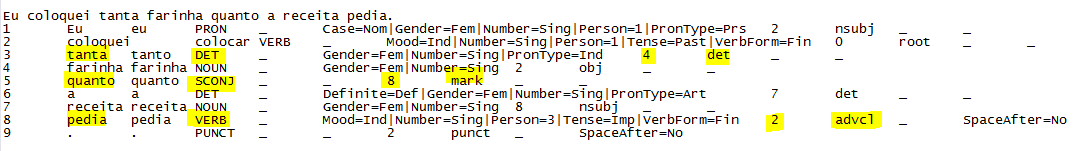
\includegraphics[width=\textwidth,height=\textheight,keepaspectratio]{imagesDrive/image20.png}
    \caption{Eu coloquei \emph{tanta farinha quanto} a receita pedia}
    \label{fig:comparative1}
    \end{figure}{}

\begin{figure}
    \centering
    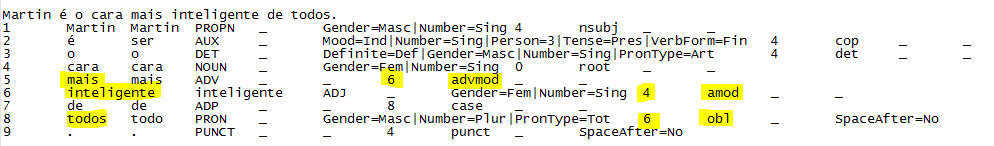
\includegraphics[width=\textwidth,height=\textheight,keepaspectratio]{imagesDrive/image27.png}
    \caption{Martin é o cara \emph{mais inteligente de todos}}
    \label{fig:comparative2}
\end{figure}{}

\subsection{Frases do Bosque-UD}



\chapter*{Abreviações}

\hyperlink{toc}{Ir para tabela de conteúdos\\}



\chapter*{Agradecimentos}

\hyperlink{toc}{Ir para tabela de conteúdos\\}



\printbibliography[heading=subbibliography,notkeyword=this]

\end{document}
